\documentclass{article}
\usepackage[utf8]{inputenc}
\usepackage[portuguese]{babel}
\usepackage{csquotes}
\usepackage{graphicx}
\usepackage{adjustbox}
\usepackage{lipsum}
\usepackage[backend=biber,autolang=other,
  bibencoding=utf8,style=alphabetic,
  ibidtracker=true]{biblatex}
\addbibresource{villard-de-honnecourt.bib}

\title{Villard de Honnecourt, o desenhador}
\date{17 de Dezembro de 2014}
\author{João Távora \\Faculdade de Belas Artes da Universidade de Lisboa}

\begin{document}

\maketitle

\section{Sinopse}

O presente trabalho é um estudo preliminar sobre Villard de
Honnencourt, arquitecto francês da primeira metade do séc XIII, a
partir do seu único legado artístico conhecido, um conjunto de notas e
desenhos sobre artes manuais, encadernados pelo próprio Villard num
caderno deixado na loja profissional a que pertencia. O trabalho
debruça-se sobre os aspectos biográfico e artístico evidenciados neste
caderno. O primeiro sustenta-se primariamente num ensaio de Teresa
Frisch \cite{teresa}, e em referências secundárias dele
extraídas. Para o segundo focou-se o livro ``Arte e Ilusão'' de
E.H. Gombrich \cite{gombrich}.

\section{Palavras-chave}

Desenho, Villard de Honnecourt, Idade Média

\section{Introdução}

De Villard de Honnecourt sobrevivem hoje 33 folhas de pergaminho
contendo desenhos e notas, datando de uma fatia razoavelmente pequena
da primeira metade do séc XII. Guardado actualmente na
\emph{Bibliothèque Nationale} em Paris, o caderno abarca uma
quantidade impressionante de temas. A variedade dos assuntos
abordados, desde notas sobre arquitectura, mecanismos de guerra,
natureza e figura humana, tornam difícil a atribuição de um propósito
único à obra. A natureza confusa da organização, intercalando desenhos
sobre uma temática com notas soltas sobre outra, intensifica esta
dificuldade e valeu ao caderno de Villard de Honnecort comparações com
os \emph{codices} de Leonardo Da Vinci \cite{teresa}.

Dado o pouco que se escreveu e se conhece deste arquitecto viajado
pela Europa, é interessante interrogarmo-nos sobre as maneira em que
esta obra seduz quem sobre ela se debruça. Em primeiro lugar está a
singularidade da obra no seu formato, conteúdo e lugar histórico. Em
segundo, coloca-se o enigma do homem que a escreveu. Ao abrir o
caderno Villard de Honencourt saúda, na terceira pessoa, o
leitor. Roga-lhe antes de nada que o recorde e que encontre utilidade
prática nos conselhos legados sobre a ``grande arte da construção'' e
sobre a ``arte do desenho''. Em relação a esta última, qualquer
inspecção sumária não defrauda esta expectativa: em todas as páginas
seguintes encontra-se uma invenção gráfica fora de série, seja no
desenho de flamingos ou das capelas radiantes de uma catedral
cisterciense.

No texto que acompanha os desenhos, Villard fala ao leitor em tom
coloquial exprimindo entusiasmo pelos temas observados e momentos
vividos . A obra tem assim um carácter concentrado na pessoa no autor,
quase intimista, uma atitude rara na idade média \footnote{Sabemos,
  por exemplo, que o Abade Suger omitiu deliberadamente, dos seus
  escritos sobre a reconstrução da abadia de St. Denis, os nomes dos
  arquitectos e artífices na que nela
  participaram. \cite{calado}}. Talvez por esta razão fale através dos
séculos aos autores contemporâneos.

\section{Aspectos biográficos}

Em \cite{teresa} Teresa Frisch repassa a investigação biográfica sobre
o arquitecto francês. A primeira observação é precisamente sobre o a
apropriação do termo ``arquitecto''. Segundo \cite{pevsner}, na idade
média dos séculos XIII e XIV, os termos ``pedreiro'' e ``arquitecto''
designam, do ponto de vista técnico, a mesma actividade, sendo a
distinção feita de acordo com nível de especialização e da patente. Da
frequência de desenhos e notas sobre arquitectura, poderemos então
especular, apesar de não haver disso prova directa, que a aprendizagem
de Villard foi sobretudo a de um construtor, que terá começado como
pedreiro, e que gradualmente terá adquirido proeminência e reputação
como executante sobre-dotado e inteligente. Esta evolução tê-lo-á
levado a encomendas de maior dimensão técnica, artística ou
administrativa, a um melhor salário e a privilégios sociais
exclusivos, como a possibilidade de viajar. \cite{teresa} observa
ainda que os primeiros passos nesta progressão teriam sido mais fáceis
para um jovem nascido numa família de arquitectos distintos.

No caso de Villard, de quem não se sabem data de nascimento ou morte,
o estilo de desenho, e escolha de elementos arquitectónicos e estilo
de desenho coloca o seu período activo no na primeira parte do
séc. XIII. Pode assumir-se que terá feito a sua aprendizagem perto de
Honnecourt, aldeia perto de Cambrai na Picardia nortenha, talvez na
abadia cisterciense de Vaucelles. É interessante notar que existe uma
planta do coro desta igreja entre os desenhos do caderno.

Villard terá ainda desenhado, em conjunto com outro arquitecto, Pierre
de Corbie, o característico ambulatório com capelas radiantes de uma
igreja cisterciense, bem como a planta do presbitério e uma planta
completa de outras duas igrejas cistercienses (\cite{teresa} e
\cite{hahnloser}). Pode então especular-se que Villard terá trabalhado
para esta ordem. Entre as encomendas estará possivelmente a catedral
de Cambrai, cuja construção foi interrompida em 1231. Villard terá
participado numa fase já avançada da contrução, já que exprime
preocupação pelo estado da mesma, numa página onde se desenham
detalhes da catedral de Reims.

De Reims, Villard viaja para a Hungria, uma viagem que menciona em
várias ocasiões. Não se sabe o propósito profissional desta viagem,
mas admite-se que se tratasse de uma encomenda advinda da sua
associação com a ordem de Cister. A única reminiscência artística da
viagem é um desenho do mosaico da igreja.

Terá talvez sido a caminho da Hungria que Villard realizou os desenhos
das torres da catedral de Laon e pormenores das fachadas das catedrais
de Chartres de Lausanne.

É geralmente assumido \cite{teresa} que Villard terá regressado da
Hungria antes da invasão tártara de 1241 e que terá passado o resto da
sua vida na Picardia, talvez como mestre de loja \footnote{Por esta
  razão, chama-se ao portefólio de desenhos ``livro de loja''
  \cite{teresa}.} na igreja de St. Quentin, onde se viria a construir
uma das maiores abadias do séc. XIII viria a ser construida.

\section{O caderno de Desenhos}

A par das competência gráficas, e em grande medida por via destas, o
caderno de Villard de Honnencourt revela um homem com um olhar e mente
aguçados, astuto na absorção de conhecimentos, consciente das teorias
artísticas e científicas da época, e dialogante com estas. Em
\cite{teresa}, observa-se que, a julgar pela diversidade de
temas tratados na pequena amostra chegada à actualidade, as tarefas a
que se dedicou terão sido tão numerosas, diversas e exigentes como
aquelas de que fala Vitrúvio no seu tratado de arquitectura.

Aquando da encadernação, Villard, que viria a presidir sobre loja
profissional à qual se tinha associado, acrescentou notas e
comentários. Mais tarde, viria a acrescentar desenhos técnicos
relacionados com técnicas de construção, medidas e geometria aplicada
de acordo com as necessidades de uma loja de
pedreiros. \footnote{Posteriormente, outros membros da loja, mais ou
  menos próximos de Villard, acrescentaram outras notas de desenhos ao
  portefólio. Não foram, no entanto, tocadas as observações de
  carácter estético ou a colecção de construções e invenções de
  engenharia.}

Villard abre o caderno dirigindo-se ao leitor:

\begin{quote} Villard de Honnecourt saúda-vos e exorta todos aqueles
que possam no trabalho ser auxiliados por este livro que rezem pela
sua alma e o recordem. Neste livro encontram-se bons conselhos sobre a
grande arte da construção e engenhos de carpintaria, e nele
encontrareis a arte do desenho [...] e seus princípios, assim como a
disciplina da geometria os requer e os ensina. \footnote{Tradução
  livre do autor a partir de \cite{teresa}.}
\end{quote}

\subsection{Forma e função}

Na pequena nota introdutória, Villard explica a função dual da obra:
Em primeiro lugar, adjectivada de ``grande arte'' está a função
prática e profissional da obra. Em segundo lugar está a ``arte do
desenho'' que serve a disciplina da geometria.

A estruturação contém, de forma subtil, uma importante e necessária
hierarquização típica da idade média: os discursos prático-científico
e estético estão sempre subordinados ao discurso religioso. Apesar de
aparecer em último, é no entanto notável que a``arte do desenho''
conste desta enumeração.

Os desenhos de Villard, que \cite{teresa} classifica em seis grupos,
podem agrupar-se de forma mais simples em três: (1) animais, (2)
figura humana e (3) desenhos diagramáticos.

Nesta última categoria contam-se os desenhos de arquitectura,
geometria, ornamentação e carpintaria. Prevalece neles a função
diagramática, e subsistem deles as linhas claras, firmes e desambíguas
inscritas a tinta no pergaminho. Nos comentários que acompanham
prevalece o carácter explicativo com indicações da apropriação da
forma à função:

\begin{quote}
  Quem desejar fazer um púlpito do qual se possam ler as escritura,
  contemple a melhor maneira de o fazer [...]  \cite[p. 13]{villard}
\end{quote}

\begin{quote}
  Quem desejar fazer uma caixa para o relógio, poderá ver aqui uma
  que vi numa ocasião. \cite[p. 12]{villard}
\end{quote}

\begin{quote} Se desejardes fazer uma asa satisfatória de uma cadeira
de coro verdadeiramente boa, vede esta. \cite[p. 14]{villard}
\end{quote}

\begin{quote} E o andar de cima terá que ter ameias para que ninguém
  possa passar pelo telhado. \cite[p. 20]{villard}
\end{quote}

O desenho diagramático de Villard é irrepreensível: todas as linhas são
firmes, uniformes e bem determinadas. Os pormenores são tornados
claros apenas quando necessário, recorrendo a sistemas informais, mas
eficazes, de perspectiva.

É interessante verificar que, estritamente dentro do grupo
diagramático, os desenhos são tanto mais exuberantes e imponentes,
quanto mais derivam produto da observação directa (e não de
projecto). Por outras palavras, Villard, plenamente atento à função
está igualmente consciente da forma, e da maneira como esta afecta e
se relaciona com o vazio da página. Alguns desenhos evidenciam um
contacto visual intenso e uma verdadeira empatia pelo modelo
arquitectónico. É o próprio Villard que que assim descreve o seu
desenho de uma janela da catedral de Reims (ver figura \ref{fig:20}):

\begin{figure}
\centering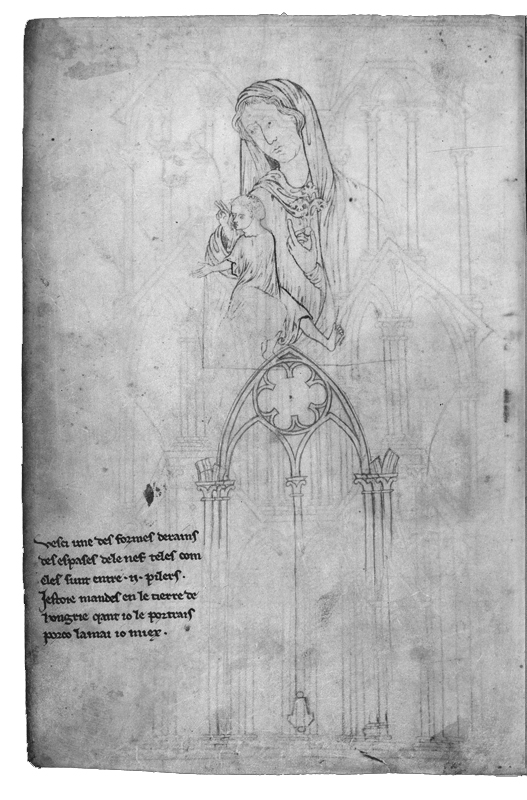
\includegraphics[height=0.6\textheight,keepaspectratio]
                          {images/20.jpg}
  \caption{Esboço de janela da catedral de Reims.}.
  \label{fig:20}
\end{figure}

\begin{quote}
Contemplai uma das janelas em Reims da [...] nave, assim como são
entre dois pilares. Mandaram-me para as terras de Hungria porque
gostei mais dela. \cite[p. 20]{villard}
\end{quote}

Não só Villard se permite temerariamente dar o seu juízo artístico
como o relaciona directamente com a possibilidade de viajar para a
Hungria. Hans Hahnloser \cite[p. 57]{hahnloser} chama a esta afirmação
``o poleiro do juízo artístico pessoal da alta idade
média''\footnote{No original ``the roost personal artistic judgment of
  the high Middle Ages'' segundo \cite{teresa}. Considerou-se a
  omissão do ``of'' uma gralha.}

\subsection{Geometrização}

Uma das primeiras coisas que salta à vista nos desenhos de figuras
humanas e animais é a sobreposição e inscrição em muitas delas de
figuras geométricas relacionadas. Em \cite[p. 130]{gombrich}, Ernst
Gombrich encontra uma explicação para este fenómeno:

\begin{quote}
  [...] the trick figures [...] included in this album of patterns. One
  could find a parallel for each of these diagrams in modern drawing
  books. Villard and his workmates must have experienced the same
  difficulties and needed the same pschological aids in learning to
  draw as we do.
\end{quote}

A explicação didáctica de Gombrich e a comparação com a ``massa de
livros que vertem da imprensa ano após ano'' \cite[p. 127]{gombrich} é
certamente admissível. É notável, de facto, como numa figura do topo
de uma das páginas \ref{caras-geometricas} encontramos a famosa
``regra de três'' para desenhar a face: mede-se a mesma distância da
eminência frontal, à eminência nasal, à base do queixo. O próprio
Villard releva o propósito pedagógico: \cite[p. 36]{villard}.

\begin{quote}
ici commence la méthode des dessins de portraiture, comme l'art de la
géométrie l'enseigne pour travailler aisément\footnote{Deve referir-se
  que os mestres de loja que mais tarde ampliaram o caderno de
  desenhos acrescentaram páginas com demonstrações de geometria
  aplicada. Em \cite{teresa}, admite-se, que isto se fica a dever ao
  método geométrico informal que Villard utiliza.}
\end{quote}

Num prévio trabalho, além de mencionar esta explicação didática
\cite[p. 17]{tavora}, analisou-se também a maneira como a geometria
serve os conceitos de ``massa'' e ``impulso'', ou seja confere
solidez, intencionalidade e credibilidade à forma, principalmente à
figura humana \cite[p. 6]{tavora}:

\begin{quote}
  Por outras palavras, a representação de sólidos geométricos no
  espaço é um problema fundamental do desenho, uma abordagem poderosa
  à sua resolução, à qual pode não bastar, por exemplo, o foco
  exclusivo na iluminação tonal ou no contorno. Segundo [Robert
    Beverly] Hale, um artista completo possui um riquíssimo
  vocabulário de possíveis geometrizações da forma, que vai
  enriquecendo ao longo da vida. O artista decide qual o sólido
  geométrico que mais lhe convém para resolver determinado
  problema. Nos retratos de Drawing Lessons... nota-se como a cabeça
  humana é representada alternadamente como oval ou paralelipípedo.
\end{quote}

Nesse trabalho, apenas o que diz estritamente respeito à ilusão da
trimensionalidade não se aplica directamente aos desenhos de Villard
de Honnecourt, que utiliza formas bidimensionais.

É precisamente esta alternância entre formas soluções geométricas que
se encontra nos desenhos de Villard de Honnecourt. Nas folhas 36 e 37,
além da exprimentação com concepções em círculo e rectângulo, Villard
utiliza uma quantidade notável de variações da concepções em estrela
para representar convincentemente várias figuras humanas perfeitamente
assentes na sinuosa linha de terra (\ref{villard-figuras-solidas}). Já
a outras figuras, como uma na página 22 em que a geometrização é menos
clara, falta esta solidez.

Estejam as formas em si explicitamente ou implicitamente
presentes\footnote{Segundo \cite{teresa}, Julius Schlosser ``observa
  claramente'' que as figuras geométricas foram sobrepostas depois de
  concebido o desenho, e não o precedem. Nota-se que tal afirmação não
  exclui que a geometria tenha estado explícita no desenho prévio
  antes da passagem a tinta \cite{calado}, ou simplemenente na mente
  do desenhador.}, a geometrização é a pedra de toque do desenho de
raíz europeia e Villard esgrime uma observação perspicaz quando
salienta a relação bidireccional entre o desenho e a geometria.

\begin{figure}
\centering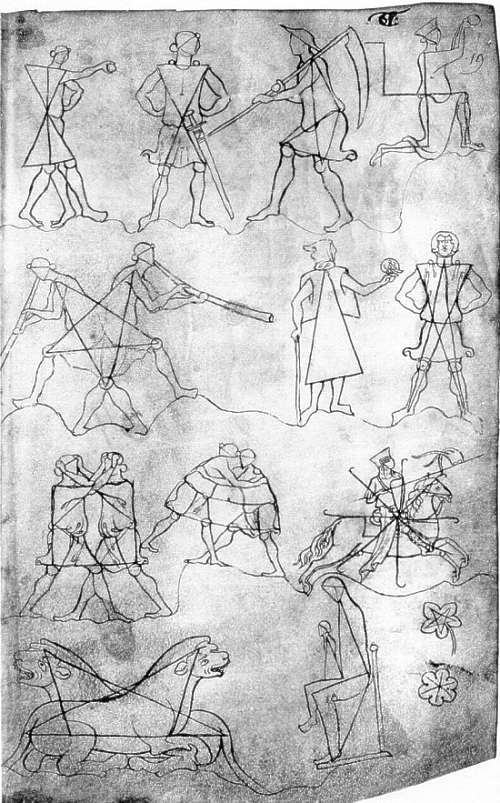
\includegraphics[height=0.6\textheight,keepaspectratio]
                          {images/villard-figuras-solidas.jpg}
  \caption{Página do portfólio de Villard De Honnecourt}.
  \label{fig:villard-figuras-solidas}
\end{figure}

\subsection{O referente ``du vif''}

De todo o caderno de desenhos de Villard de Honnecourt, recaem
invariavelmente as atenções de qualquer autor sobre a página onde se
representa um leão e um ouriço \cite[p. 20]{villard}. O desenho do
leão, que ocupa quase toda a página, é claramente estilizado,
particularmente no rosto. A perplexidade que sugere a legenda
subsequente, em que Villard diz que o desenho foi realizado à vista e
do natural, só é comparável àquela com que o rosto do leão parece
fitar o leitor (\cite[p. 48]{villard} e figura
\ref{fig:villard-leao}):

\begin{quote}
  voici un lion [...] et saves bien qu'il fut contrefait du vif
\end{quote}

\begin{figure}
\centering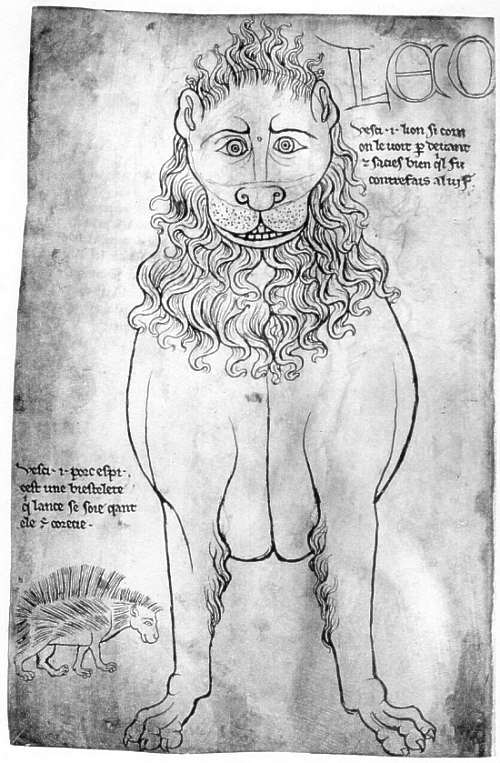
\includegraphics[height=0.6\textheight,keepaspectratio]
                          {images/villard-leao.jpg}
  \caption{Desenho de leão e ouriço}
  \label{fig:villard-leao}
\end{figure}

Ernst Gombrich analisa com detalhe a relação entre a finalidade
esquemática e ilusória da arte através da história, adverte para uma
leitura correcta do termo ``du vif'', que teriam para Villard um
significado muito diferente do que têm para um observador
contemporâneo \cite[p. 68]{gombrich}:

\begin{quote}
  He can only have meant that he drew his schema in the presence of
  the lion. How much of his actual observations he allowed to enter
  into the formula is another matter.
\end{quote}

A partir \cite{teresa}, chegamos a uma citação de \cite{schlosser},
que comunica uma interpretação igualmente cautelosa:

 \begin{quote}
  [...] without doubt Villard did not intend to dissemble when quite
  clearly he did not draw from nature, for to him 'nature' meant
  something different from what it means to us; for a man of the
  Middle Ages it was impossible to consider as meaningful anything but
  the idea, the concept, behind the appearance of things. The natural
  form was like soft wax which had to yield to the artistic invention.
 \end{quote}

Em \cite{teresa} observa-se que as figuras de Villard, no estilo
artístico vigente, têm todas ``proporções elegantes e
nobres''. Por outras palavras, o artista medieval não tenta
representar o particular, e preocupa-se com o universal. Villard não
deseja comunicar a forma \emph{daquele} leão, mas sim a própria ideia
de leão. Em \cite{gombrich}, observa-se por diversas vezes que esta é
a subordinação possível à teoria de arte vigente na época, quase
directamente apoiada na estética de Platão e em obras como ``A
República'': ao pintar um aspecto particular, o pintor está três graus
afastado da realidade. Dessa forma, o domador e tratador do leão, cujo
método Villard também se esforça por descrever nas páginas seguintes,
estará mais próximo da realidade do que qualquer desenho naturalista.

Em \cite{gombrich} estabelece-se uma ligação interessante entre arte
medieval e pós-medieval: para Gombrich, o \emph{esquema} que o artista
medieval desenha \emph{é} a imagem, sendo para que o artista
pós-medieval, ele é o ponto de partida para correcções. Ao ``sintoma''
desta atitude vir-se-á a chamar ``esboço''. \cite[p. 68]{gombrich}.

À primeira vista parece efectivamente ausente do caderno de Villard de
Honnecort a ideia de ``esboço''. Schlosser e Gombrich deixam claro que
o artista não o valorizava e prefere a idealização esquemática. No
entanto, isto não constitui evidência que o esboço, algo de subjacente
ao desenho, nunca tenha existido.

Nas páginas 35, 48 e 51 encontrar ténues linhas auxiliares (não as de
geometria) que auxiliaram a construção do desenho, algumas, como nas
páginas 5 e 35 parecem procuras falhadas. Na página 18 há um contraste
temático fortíssimo no imediatismo com que Villard escolhe o lugar
geométrico para desenhar um homem de barbas no meio de um desenho
arquitectónico. \cite[p. 18]{villard}\footnote{Esta escolha pode ser
  justificada com a disponibilidade do pergaminho, que tinha um preço
  elevado na época \cite{calado}. No entanto Villard teria espaço
  nesta página para, por exemplo colocar a figura com a orientação do
  texto, e não o fez.}, Não só Villard não consegui eliminar estas
``erros'', como é questionável se não os terá valorizado. No mínimo, é
uma evidência que há Villard, tanto em desenhos isolados como na obra
como um todo, um entusiasmo despreocupado e espontâneo no desenho. São
precisamente estas duas qualidades que gerações mais tarde virão a
valorizar nos esboços de grandes mestres.

\section{Conclusão}

É inquestionável que o propósito primário dos desenhos de Villard de
Honnecourt é prático e funcional. Consiste em ensinar um jovem
construtor a transferir pequenos desenhos preparatórios para o tamanho
final no meio que poderia ser madeira ou pedra.

Quanto à geometria, a insistência de Villard na sua relação com o
desenho indicam quão vitais seria esta disciplina para qualquer
aprendiz.

O caderno de desenhos é uma investigação entusiasmada sobre o Desenho
contada na primeira pessoa. O seu propósito declarado é, numa primeira
abordagem, puramente prático e a ele submete-se o discurso
estético. No entanto, o confronto com os próprios desenhos e a relação
de quase intimidade que se estabelece com o desenhador rapidamente
fazem ressair o carácter artístico.

Pode então especular-se que, dadas as condições propícias - carreira
próspera, viagens e o contacto com o exótico - se produziram no
caderno de Villard de Honnecourt os ``primeiros sintomas'' da
emergência do Desenho como meio estético autónomo.

\printbibliography[heading=bibliography,title={Bibliografia},type=book]

\end{document}
